\section*{Section \ref{S:equivclasses} Equivalence Classes}

\begin{enumerate}
\item \begin{enumerate}
\item Use the directed graph to examine all the cases necessary to prove that $\sim$ is an equivalence relation.

\item $\left[ a \right] = \left[ b \right] = \left\{ a,b \right\}$; $\left[ c \right] = \left\{ c \right\}$; $\left[ d \right] = \left[ e \right] = \left\{ d,e \right\}$.
\end{enumerate}



\item Followingis the directed graph for this equivalence relation.
\begin{figure}[h]
\begin{center}
\scalebox{0.8}{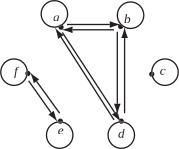
\includegraphics{figps-exer2-73.eps}}
\end{center}
\end{figure}

The equivalence class are
\[
[a] = [b] = [d] = \{a, b, d \}, \quad [c] = \{ c \}, \quad [e] = [f] = \{ e, f \}.
\]



\item Let   $A = \left\{ {0, 1, 2, 3,  \ldots , 999, 1000} \right\}$.  Define the relation  $R$  on  $A$  as follows:  For  $x, y \in A$,  $x \mathrel{R} y$ if and only if  $x$  and  $y$  have the same number of digits.

Let $x \in A$.  Since $x$ has the same number of digits as itself, the relation $\mathrel{R}$ is reflexive.  Now let $x, y, z \in A$.  If $x \mathrel{R} y$, then $x$  and  $y$  have the same number of digits.  Hence, $y$ and $x$ have the same number of digits and $y \mathrel{R} x$, and so $\mathrel{R}$ is symmetric.

If $x \mathrel{R} y$ and $y \mathrel{R} z$, then $x$  and  $y$  have the same number of digits and 
$y$  and  $z$  have the same number of digits.  Hence, $x$  and  $z$  have the same number of digits, and so $x \mathrel{R} z$.  Therefore, $\mathrel{R}$ is transitive.

The equivalence classes are:  
$\left\{ 0, 1, 2, \ldots , 9 \right\}$, $\left\{ 10, 11, 12, \ldots , 99 \right\}$, \\
$\left\{ 100, 101, 102, \ldots , 999 \right\}$, $\left\{ 1000 \right\}$.



\item The congruence classes for the relation of congruence modulo 5 on the set of integers are:

\begin{multicols}{2}$\left[ 0 \right] = \left\{ 5n \mid n \in \mathbb{Z} \right\}$

$\left[ 1 \right] = \left\{ 5n +1 \mid n \in \mathbb{Z} \right\}$

$\left[ 2 \right] = \left\{ 5n + 2 \mid n \in \mathbb{Z} \right\}$

$\left[ 3 \right] = \left\{ 5n + 3 \mid n \in \mathbb{Z} \right\}$

$\left[ 4 \right] = \left\{ 5n + 4 \mid n \in \mathbb{Z} \right\}$
\end{multicols}


\item \begin{enumerate}
\item Let $a, b, c \in \Z_9$.  Since $a^2 \equiv a^2 \pmod 9$, we see that $a \sim a$ and $\sim$ is reflexive.  Also, if $a \sim b$, then $a^2 \equiv b^2 \pmod 9$ and hence, by the symmetric property of congruence, $b^2 \equiv a^2 \pmod 9$.  This proves that $\sim$ is symmetric.  Finally, if $a \sim b$ and $b \sim c$, then 
$a^2 \equiv b^2 \pmod 9$ and $b^2 \equiv c^2 \pmod 9$.  By the transitive property of congruence, we conclude that $a^2 \equiv c^2 \pmod 9$ and hence, $a \sim c$.  This proves that $\sim$ is transitive.  The distinct equivalence classes are
\[
\{ 0, 3, 6 \}, \quad \{ 1, 8 \}, \quad \{2, 7 \}, \quad \{4, 5 \}.
\]
\item The proof that $\approx$ is an equivalence relation on $\Z_9$ is similar to the proof in Part~(a) that $\sim$ is an equivalence relation on $\Z_9$.  The distinct equivalence classes for $\approx$ are
\[
\{ 0, 3, 6 \}, \quad \{ 1, 4, 7 \}, \quad \{2, 5, 8 \}.
\]
\end{enumerate}



\item \begin{enumerate}
\item Let $x \in \left[ \dfrac{5}{7} \right]$.  Then $x - \dfrac{5}{7} \in \Z$, which means that there is an integer $m$ such that $x - \dfrac{5}{7} = m$, or $x = \dfrac{5}{7} + m$.  This proves that \linebreak
$x \in \left\{ \left. m + \dfrac{5}{7} \right| m \in \Z \right\}$ and, hence, that
$\left[ \dfrac{5}{7} \right] \subseteq \left\{ \left. m + \dfrac{5}{7} \right| m \in \Z \right\}$.

Now let $y \in \left\{ \left. m + \dfrac{5}{7} \right| m \in \Z \right\}$.  So there exists an integer $m$ such that $y = m + \dfrac{5}{7}$.  This means that $y - \dfrac{5}{7} = m$ and hence, $y - \dfrac{5}{7} \in \Z$.  Therefore, $y \sim \dfrac{5}{7}$, which means that $y \in \left[ \dfrac{5}{7} \right]$ and 
$\left\{ \left. m + \dfrac{5}{7} \right| m \in \Z \right\} \subseteq \left[ \dfrac{5}{7} \right]$.

\item If $a \in \Z$, then $[a] = \Z$.

\item Define $f\x \Z \to \left[ \dfrac{5}{7} \right]$ by $f(m) = m + \dfrac{5}{7}$ for each $m \in \Z$.  To prove $f$ is an injection, let $m, n \in \Z$ and assume that 
$f(m) = f(n)$.  Then $m + \dfrac{5}{7} = n + \dfrac{5}{7}$, which implies that $m = n$.  Therefore, $f$ is an injection.  To prove that $f$ is a surjection, let 
$y \in  \left[ \dfrac{5}{7} \right]$.  By Part~(a), there exists an $m \in \Z$ such that 
$y = m + \dfrac{5}{7}$.  We then see that $f(m) = y$ and $f$ is a surjection.
\end{enumerate}


\item \begin{enumerate}
\item If $x \in \R$, then $x - x = 0$ and hence, $x \sim x$.  So the relation $\sim$ is reflexive.  Now let $x, y \in \R$ and assume that $x \sim y$.  Then $x - y \in \Q$ and hence, $-(x - y) \in \Q$.  This means that $y - x \in \Q$ and hence, $y \sim x$.  Therefore, $\sim$ is symmetric.  Now let $x, y, z \in \R$ and assume that $x \sim y$ and 
$y \sim z$.  Then $x - y \in \Q$ and $y - z \in \Q$.  We can then conclude that 
$(x - y) + (y - z) \in \Q$ or that $x - z \in \Q$.  Hence, $x \sim z$ and the relation 
$\sim$ is transitive.

\item The following real numbers are in $\left[ \sqrt{2} \right]$:  $\sqrt{2}$, 
$1 + \sqrt{2}$, $-1 + \sqrt{2}$, $\dfrac{1}{2} + \sqrt{2}$, $\dfrac{2}{3} + \sqrt{2}$.

\item If $a \in \Q$, then $[a] = \Q$.

\item Let $x \in \left[ \sqrt{2} \right]$.  Then $x - \sqrt{2} \in \Q$, which means that there is a rational number $q$  such that $x - \sqrt{2} = q$, or $x = \sqrt{2} + q$.  This proves that $x \in \left\{ \left. r + \sqrt{2} \right| r \in \Q \right\}$ and, hence, that
$\left[ \sqrt{2} \right] \subseteq \left\{ \left. r + \sqrt{2} \right| r \in \Q \right\}$.

Now let $y \in \left\{ \left. r + \sqrt{2} \right| r \in \Q \right\}$.  So there exists a rationalnumber  $r$ such that $y = r + \sqrt{2}$.  This means that $y - \sqrt{2} = r$ and hence, $y - \sqrt{2} \in \Q$.  Therefore, $y \sim \sqrt{2}$, which means that 
$y \in \left[ \sqrt{2} \right]$ and 
$\left\{ \left. r + \sqrt{2} \right| r \in \Q \right\} \subseteq \left[ \sqrt{2} \right]$.

\item Define $f\x \Q \to \left[ \sqrt{2} \right]$ by $f(r) = r + \sqrt{2}$ for each $r \in \Q$.  To prove $f$ is an injection, let $p, r \in \Q$ and assume that 
$f(p) = f(r)$.  Then $p + \sqrt{2} = r + \sqrt{2}$, which implies that $p = r$.  Therefore, $f$ is an injection.  To prove that $f$ is a surjection, let 
$y \in  \left[ \sqrt{2} \right]$.  By Part~(d), there exists an $r \in \Q$ such that 
$y = r + \sqrt{2}$.  We then see that $f(r) = y$ and $f$ is a surjection.
\end{enumerate}


\item For this equivalence relation,
\begin{align*}
[0] &= \{ 5m \mid m \in \Z \} & [1] &= \{ 5m + 1 \mid m \in \Z \} \\
[2] &= \{ 5m + 2 \mid m \in \Z \}  &  [3] &= \{ 5m + 3 \mid m \in \Z \} \\
[4] &= \{ 5m + 4 \mid m \in \Z \}
\end{align*}



\item $A = \mathbb{Z} \times \left( {\mathbb{Z} - \left\{ 0 \right\}} \right)$.  For  
$\left( {a, b} \right), \left( {c, d} \right) \in A$,  
$\left( {a, b} \right) \approx \left( {c, d} \right)$ if and only if  $ad = bc$.

\begin{enumerate}
\item Let $\left( a, b \right) \in A$.  Since $ab = ba$, we see that 
$\left( a, b \right) \approx \left( a, b \right)$, and hence, $\approx$ is reflexive.

Now let $\left( a, b \right), \left( c, d \right) \in A$ and assume that 
$\left( a, b \right) \approx \left( c, d \right)$.  Then, $ad = bc$.  Hence, $cb = da$ and 
$\left( c, d \right) \approx \left( a, b \right)$.  Therefore, $\approx$ is symmetric.

Finally, let $\left( a, b \right), \left( c, d \right), \left( m, n \right) \in A$ and assume that 
$\left( a, b \right) \approx \left( c, d \right)$ and that 
$\left( c, d \right) \approx \left( m, n \right)$.  We conclude that
\begin{center}
$ad = bc$ and $cn = dm$.
\end{center}
We multiplby both sides of the first of these equations by $n$ to obtain $adn = bcn$.  We then subsitute $cn = dm$ on the right side of this equation to obtain
\[
adn = bdm.
\]
Since $d \ne 0$, we cancel $d$ from both sides of this equation to obtain $an = bm$.  This proves that $\left( a, b \right) \approx \left( m, n \right)$, and hence, $\approx$ is transitive.

\item In the proof that $\approx$ is an equivalence relation, we needed to have $d \ne 0$ to be able to cancel this from both sides of an equation.  This is why it was necessary to assume that second coordinate in the ordered pairs in $A$ are not zero.

\item $\left( a, b \right) \approx \left( 2, 3 \right)$ if and only if  $3a = 2b$.


\item $\left( a, b \right) \in \left[ \left( 2, 3 \right) \right]$ if and only if $3a = 2b$.  All examples must satisfy this equation.

\item $\left[ \left( 2, 3 \right) \right] = \left\{ \left( a, b \right) \in A \mid 3a = 2b \right\}$.
\end{enumerate}



\item The result stated in the exercise is incorrect.  The relation $\sim$ is not an equivalence relation.  It can be redefined to be an equivalence relation as follows:
\begin{center}
For $x, y \in \R$, $x \sim y$ if and only if either $x = 0$ and $y = 0$ or $xy > 0$.
\end{center}
In this case, the equivalence classes are
\[
\{ 0 \}, \quad \{ x \in \R \mid x > 0 \}, \quad \{ x \in \R \mid x < 0 \}.
\]



\item \begin{enumerate}
\item $[ (0, 0) ] = \{ (0, 0) \}$.

\item $[ (2, 3) ] = \{ (x, y) \in \R \times \R \mid x^2 + y^2 = 13$.  This equivalence class consists of the points in the plane on a circle of radius $\sqrt{13}$ centered at the origin.

\item Except for $[(0, 0)]$, the equivalence classes for this equivalence relation consist of points on a circle whose center is the origin.

\item Let $C_0 = \{ (0, 0) \}$ and for each positive real number $r$, let $C_r$ be the set of points on the circle of radius $r$ whose center is at the origin.  Then
\[
C_r = [ (r, 0) ].
\]
Now let $(a, b) \in \R \times \R$ and let $r = \sqrt{a^2 + b^2}$.  Then, $[a, b] = [r, 0]$ and so the set of all equivalence classes of $\sim$ is 
\[
T =  \{ C_r \mid r \in \R^* \}.
\]
Now define $f\x \R^* \to T$ by $f(r) = C_r$.  The work above shows that $f$ is a surjection.  So let $r, s \in \R^*$ and assume that $f(r) = f(s)$.  This means that 
$C_r = C_s$ and this implies that $r^2 = s^2$ or that $r = s$.  So the function $f$ is an injection.
\end{enumerate}





\item \begin{enumerate}
\item For each  $a, b \in A$,    $a\nsim b$ if and only if   
        $\left[ a \right] \cap \left[ b \right] = \emptyset $.

\textbf{\emph{Proof}.}  If $a\nsim b$, then $\left[ a \right] \ne \left[ b \right]$.  Hence, by Theorem~\ref{T:propsofequivclasses}, $\left[ a \right] \cap \left[ b \right] = \emptyset $.  In addition, if $a \sim b$, then by Theorem~\ref{T:propsofequivclasses}, 
$\left[ a \right] = \left[ b \right]$ and so, 
$\left[ a \right] \cap \left[ b \right] \ne \emptyset $.  This proves that if $a \sim b$, then , $\left[ a \right] \cap \left[ b \right] \ne \emptyset $ and hence that if 
$\left[ a \right] \cap \left[ b \right] = \emptyset $, then $a \nsim b$.

\item Statement~(3) in Theorem~\ref{T:propsofequivclasses} is logically equivalent to, 
``For each  $a, b \in A$,   if  $\left[ a \right] \ne \left[ b \right]$, then   
$\left[ a \right] \cap \left[ b \right] = \emptyset $.''  This uses the following logical equivalency:  $\mynot P \vee Q \equiv P \to Q$.

\item This is the contrapositive of the statement in~(b).
\end{enumerate}
\end{enumerate}


\subsection*{Explorations and Activities}
\setcounter{oldenumi}{\theenumi}
\begin{enumerate} \setcounter{enumi}{\theoldenumi}
\item Let  $A = \left\{ {a, b, c, d, e} \right\}$ and let  
$\mathcal{C} = \left\{ {\left\{ {a, b, c} \right\}, \left\{ {d, e} \right\}} \right\}$. 

\begin{enumerate}
\item $\mathcal{C}$ is a partition of $A$  since each set in  $\mathcal{C}$  is nonempty, each element of  $A$  is in one set contained in  $\mathcal{C}$ , and the two unequal subsets  of  $A$  contained in  $\mathcal{C}$  are disjoint.

\item Let  $x \in A$.  Then ,  $x \sim x$ since there exists a set  $T$  in  $\mathcal{C}$  such that  $x \in T$ and  $x \in T$.  This means that the relation  $\sim$  is reflexive on  $A$.
\vskip6pt
Now let  $x, y \in A$ and assume that  $x \sim y$.  Then, there exists a set  $T$  in  
$\mathcal{C}$  such that  $x \in T$ and  $y \in T$.  But then,  $y \in T$ and  $x \in T$, and hence,  $y \sim x$.  Therefore, the relation  $\sim$  is symmetric.
\vskip6pt

Finally, let  $x, y, z \in A$  and assume that  $x \sim y$  and  $y \sim z$.  Then, there exists a set  $T$  in  $\mathcal{C}$  such that  $x \in T$ and  $y \in T$  and  there exists a set  $V$  in  $\mathcal{C}$  such that  $y \in V$ and  $z \in V$.  Since  $y \in T \cap V$, we can conclude that  $T \cap V \ne \emptyset $.  Since  $T$  and  $V$  are sets in the partition  $\mathcal{C}$ , this implies that  $T = V$.  Therefore,  $x \in T$ and  $z \in T$ and hence, the relation  $\sim$  is transitive. So, we have proven that  $\sim$  is an equivalence relation on  $A$.
\vskip6pt

The equivalence classes for $\mathcal{C}$ are:  $\left[ a \right] = \left[ b \right] = \left[ c \right] = \left\{ {a, b, c} \right\}$  and   
$\left[ d \right] = \left[ e \right] = \left\{ {d, e} \right\}$.  These are the same subsets of 
$A$ that form the partition $\mathcal{C}$.


\item Repeat the proof in Part (b).

\item Let  $a \in A$  and let  $T \in \mathcal{C}$ such that  $a \in T$.  Now assume that  
$x \in \left[ a \right]$.  Then,  $x \sim a$ and hence,  there exists a set  $V$  in  
$\mathcal{C}$  such that  $x \in V$ and  $a \in V$.  Since  $a \in T \cap V$, we know that  
$T \cap V \ne \emptyset $, and  since  $T$  and  $V$  are sets in the partition  $\mathcal{C}$, this implies that  $T = V$.   Therefore, $x \in T$, and we conclude that  
$\left[ a \right] \subseteq T$.

Now let  $x \in T$.  Then by the definition of  $\sim$,  $x \sim a$ and  
$x \in \left[ a \right]$.  This proves that  $T \subseteq \left[ a \right]$ and hence that  
$\left[ a \right] = T$.
\end{enumerate}



\item Let $I$ be the identity matrix in $\mathcal{M}_{n, n}\left( \R \right)$.
\begin{enumerate}
\item For $A \in \mathcal{M}_{n, n}\left( \R \right)$, $A = IAI^{-1}$ and so $A \sim A$.  Hence, the relation $\sim$ is reflexive.  

Now let $A, B, C \in \mathcal{M}_{n, n}\left( \R \right)$.  First assume that $A \sim B$.  Then there exists an invertible matrix $P$ in $\mathcal{M}_{n, n}\left( \R \right)$ such that $B = PAP^{-1}$.  From linear algebra, we know that $P^{-1}$ is invertible and so
\begin{align*}
P^{-1}BP &= P^{-1} \left( PAP^{-1} \right) P \\
         &= \left( P^{-1}P \right) A \left( P^{-1} P \right) \\
         &= A.
\end{align*}
Hence, $B \sim A$ and the relation $\sim$ is symmetric.  Now assume that $A \sim B$ and 
$B \sim C$.  Then there exist invertible matrices $P$ and $Q$ in 
$\mathcal{M}_{n, n}\left( \R \right)$ such that $B = PAP^{-1}$ and $C = QBQ^{-1}$.  We then see that
\begin{align*}
C &= Q \left( PAP^{-1} \right) Q^{-1} \\
  &= \left(QP \right) A \left( P^{-1} Q^{-1} \right) \\
  &= \left( QP \right) A \left( QP \right)^{-1}.
\end{align*}
This proves that the relation $\sim$ is transitive and hence, $\sim$ is an equivalence relation.

\item Let $A, B, C \in \mathcal{M}_{n, n}\left( \R \right)$.  Since $\det(A) = \det(A)$, we see that $A \mathrel{R} A$ and $R$ is reflexive.  In addition, if $\det(A) = \det(B)$, then $\det(B) = \det(A)$.  This can be used to prove that $R$ is symmetric.  Finally, if 
$\det(A) = \det(B)$ and $\det(B) = \det(C)$, then $\det(A) = \det(C)$.  This can be used to prove that $R$ is transitive.

\item For this problem, $\sim$ is an equivalence relation on $\R$. Let $A, B, C \in \mathcal{M}_{n, n}\left( \R \right)$.  Since $\det(A) \in \R$ and $\sim$ is reflexive, 
$\det(A) \sim \det(A)$.  This proves that $\approx$ is reflexive on 
$\mathcal{M}_{n, n}\left( \R \right)$.  Now assume that $A \approx B$.  Then $\det(A) \sim \det(B)$.  Since $\sim$ is symmetric, we conclude that $\det(B) \sim \det(A)$ and hence, 
$B \approx A$.  This proves that $\approx$ is symmetric.

Finally, assume that $A \approx B$ and $B \approx C$.  Then $\det(A) \sim \det(B)$ and 
$\det(B) \sim \det(C)$.  Since $\sim$ is transitive, we can conclude that 
$\det(A) \sim \det(C)$.  Hence, $A \approx C$ and so $\approx$ is transitive.  This proves that $\approx$ is an equivalence relation on $\mathcal{M}_{n, n}\left( \R \right)$.
\end{enumerate}

\end{enumerate}
\hbreak
\endinput
